\chapter{Presentación del problema}
Durante 2019 se entrevistó al Dr. Mario Alberto Rios Macias Jefe del Área de Morfología de la Escuela Superior de Medicina (ESM) 
del Instituto Politécnico Nacional (IPN) y comentó que \textbf{“Los medios que se utilizan para el estudio del cuerpo humano principalmente 
son medios impresos tradicionales, así como el uso de cuerpos para su disección y análisis posterior”.}\\
El uso de cuerpos para su disección tiene un alto costo
%(ver tabla o apartado, información que se describe más adelante)
que incluye el mantenimiento del cuerpo en las instalaciones, el mantenimiento de las instalaciones, y la inhumación de los cuerpos.\\
Por lo tanto, se encuentra en esta disciplina o área una oportunidad importante que podría acercar la tecnología en el alumnado … 

\section{Contexto y motivación}

\section{Departamento de Morfología ESM del IPN}

\section{Objetivos del Sistema}
Analizar, diseñar, desarrollar y probar un prototipo de sistema que utiliza la tecnología de Realidad Virtual, para ofrecer una experiencia orientada al estudio 
de la anatomía y morfología del cuerpo humano, específicamente del sistema digestivo.\\
\subsection{Objetivos Específicos}
\begin{itemize}
	\item Utilizar como insumo para la elaboración de los modelos, las referencias documentales y confiables que proporcionan los expertos del área de morfología de la ESM del IPN sobre el sistema digestivo.
	\item Elaboración de modelos en tres dimensiones del sistema digestivo humano
	\begin{itemize}
		\item Glándulas Salivales
		\item Cavidad Oral
		\item Faringe
		\item Esófago
		\item Estómago
		\item Intestino Delgado
		\begin{itemize}
		  \item Hígado
		  \item Páncreas
		  \item Vesícula Biliar
		\end{itemize}
		\item Intestino Grueso y Ano  
	  \end{itemize}
	\item Diseñar y desarrollar
	\item Probar los componentes de software del sistema y realizar su interacción con los elementos de hardware que propiamente proporcionan el entorno de  Realidad Virtual.	
\end{itemize}

\section{Revisión del Estado del Arte}
A continuación se muestran algunos de trabajos académicos desarrollados en México y fueron comparados con el trabajo planeado. Como comparativa y de forma ilustrativa 
del sector académico.\\
\newline
\begin{enumerate}
\item TT No. 2014-A058 “Sistema para la orientación de los efectos sobre la espalda humana en pacientes con sobrepeso”\cite{tt1}
\item TT No. 2012-B055 “Laboratorio Virtual del cuerpo humano 3D con asistente de ayuda en línea para el nivel superior bajo el paradigma de Educación Basada en Web con 
tecnologías de Web Semántica”\cite{tt2}
\item TT No. 2014-B035 “Simulación en Tercera Dimensión del Sistema Circulatorio de los Cánidos para el uso Educativo”\cite{tt3}
\item TT No. 2014-B039 “Simulación de una Línea del Metro con Realidad Virtual”\cite{tt4}
\item Tesis que para optar por el grado de Maestro en Ciencia e Ingeniería de la Computación, Sistema de seguimiento de movimiento de las extremidades superiores basado 
en sensores inerciales para rehabilitación en realidad virtual.\cite{mastersthesis1}
\item Adecuación educativa de la realidad virtual como herramienta didáctica para el proceso enseñanza-aprendizaje / tesis que para obtener el título de Licenciado en 
Pedagogía, presenta Maria de la O García Noriega; asesor Lucina Moreno Valle Suárez.\cite{te1}
\end{enumerate}
Así mismo se ha encontrado software propietario desarrollado por empresas privadas los cuales son los siguientes.\\
\begin{itemize}
\item The Body VR: Anatomy Viewer es la única herramienta de visualización de Realidad Virtual disponible en el mercado que se basa en datos médicos específicos del 
paciente (por ejemplo, MRI, CT, PET) y cumple con los estándares DICOM. Proporciona simulaciones de R.V. anatómicas en tiempo real para visualizar diagnósticos médicos, 
ilustrar el impacto de los procedimientos y tratamientos, y crear una toma de decisiones más educada.\
\begin{figure}[H]
	\begin{center}
 		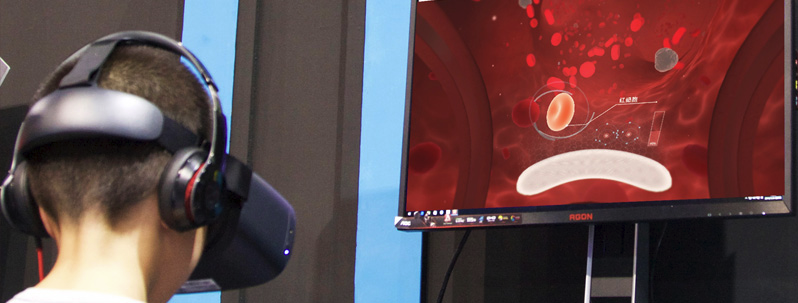
\includegraphics[width = 0.5\textwidth]{source/images/image9.png}
 		\captionof{figure}{\label{fig:ea1}Software “The Body VR” en uso.}
	\end{center} 
\end{figure}
\item Anatomyou VR: Estructuras anatómicas fotorrealistas, modeladas en colaboración con RenderArea, validadas por expertos clínicos y certificadas por personal capacitado 
en  Tecnologías Médicas de la Universidad de Las Palmas de Gran Canaria.
\begin{figure}[H]
	\begin{center}
 		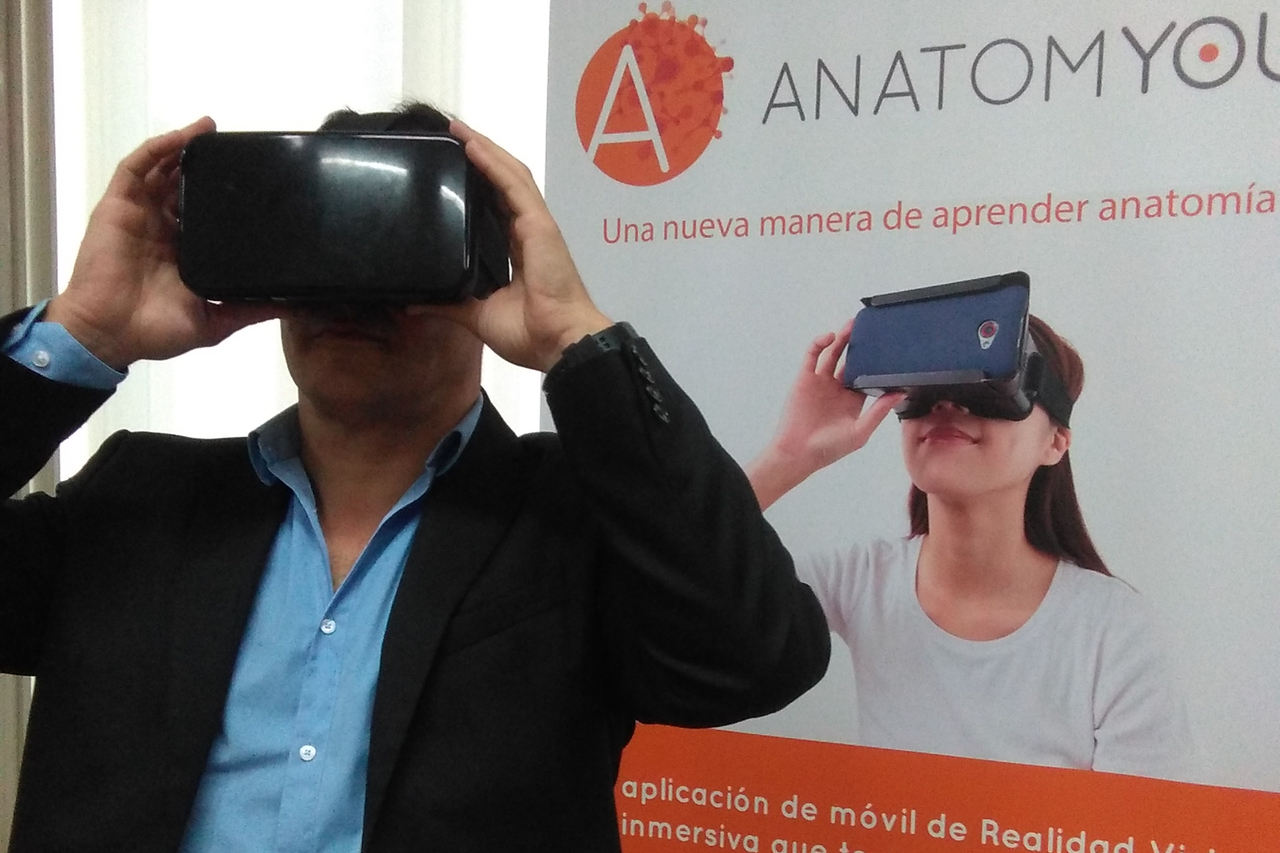
\includegraphics[width = 0.5\textwidth]{source/images/image59.png}
 		\captionof{figure}{\label{fig:ea2}Pancarta promocional de “Anatomyou VR}
	\end{center} 
\end{figure}
\item Biodigital Anatomy: El cuerpo tridimensional más completo, científicamente preciso e interactivo jamás ensamblado. Anatomía masculina y femenina, en los detalles 
básicos (gratuitos) y profesionales. Cada sistema está completamente segmentado, etiquetado y direccionable para una fácil configuración que satisfaga cualquier necesidad educativa.
\begin{figure}[H]
	\begin{center}
 		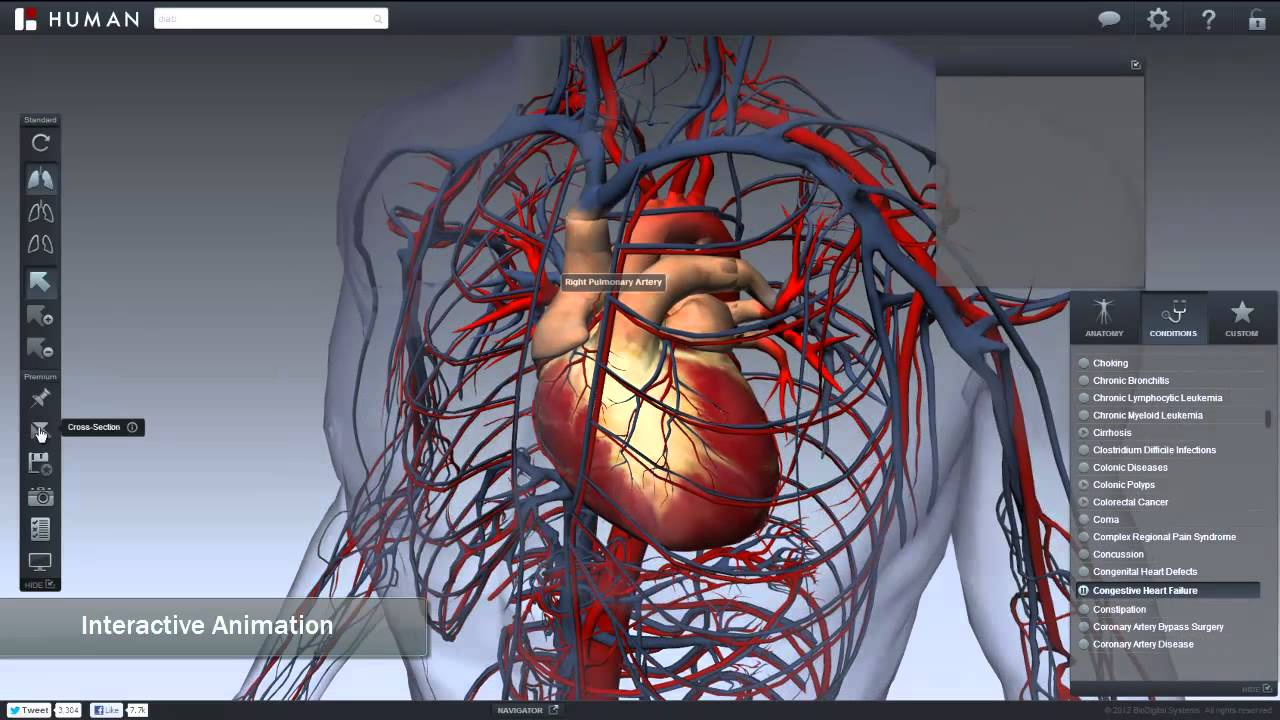
\includegraphics[width = 0.5\textwidth]{source/images/image18.png}
 		\captionof{figure}{\label{fig:ea3}Interfaz del software de Biodigital Anatomy}
	\end{center} 
\end{figure}
\item 3D Organon VR Anatom: 3D Organon es un completo atlas anatómico que presenta los 15 sistemas del cuerpo humano. Incluye más de 4,000 estructuras y órganos anatómicos 
realistas y más de 160 correlaciones clínicas encontradas por sistema del cuerpo.
\begin{figure}[H]
	\begin{center}
 		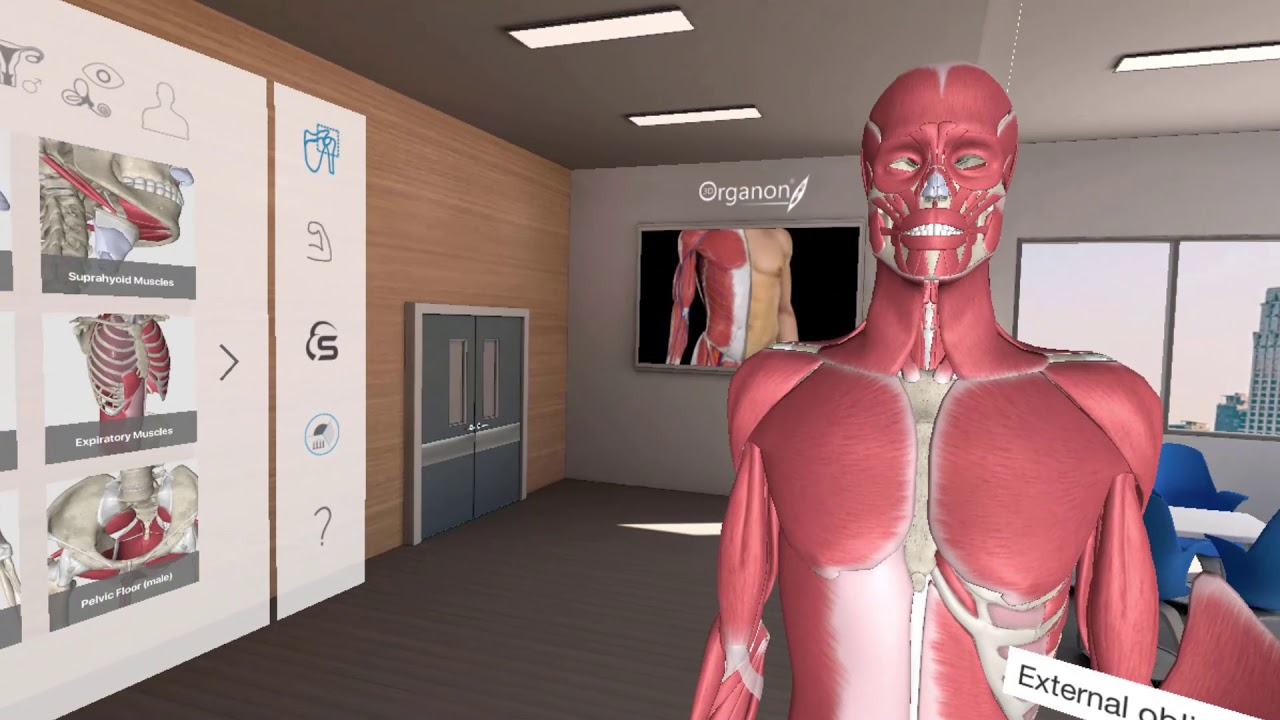
\includegraphics[width = 0.5\textwidth]{source/images/image5.png}
 		\captionof{figure}{\label{fig:ea4}Interfaz del software de 3D organon VR Anatom}
	\end{center} 
\end{figure}
\end{itemize}

\section{Organización de capítulos}
Este documento es el reporte técnico final del trabajo terminal titulado “Sistema de Realidad Virtual del Cuerpo Humano para el Estudio del Sistema Digestivo” con número de registro TT: 2019-A104.

En el \textbf{Capítulo} I se habla del problema identificado, por qué se considera como tal y cómo es que se ayudó a resolver el problema planteado mediante la ingeniería en sistemas computacionales. También se menciona que se obtiene al concluir con este trabajo terminal, tales como el prototipo del sistema.\\

En el \textbf{Capítulo II Marco Conceptual} se mostrarán todos los diagramas y documentos generados al analizar y generar un diseño del sistema que se estará desarrollando. Aquí se encuentra la arquitectura general del sistema, y los modelos gráficos de apoyo presentados en el Análisis Estructurado Moderno.\\

En el \textbf{Capítulo III Diseño} se describe el trabajo generado en el desarrollo del documento hasta el mes de mayo de 2020 para TT2.\\

En el \textbf{Capítulo IV Verificación y Pruebas} se muestran pruebas hechas sobre las implementaciones del sistema siguiendo un guión para la prueba.\\
 
En el \textbf{Capítulo V Conclusión} se muestran los resultados obtenidos y experiencias para mejorar el proceso, así como la vertiente para continuar con el trabajo y las conclusiones del integrante.\\

Finalmente, se encuentran las Referencias de todos los recursos empleados para dar soporte y estructura a este Trabajo Terminal, y en los apéndices se anexan elementos extra que dan información más detallada sobre lo que aquí fue realizado.\\
